	For a motivating example, we will borrow data from Hoel and Walberg (1972). In this tumorigenicity study, 96 RFM mice (a discontinued line of mice which were at high risk for tumors) are exposed to a conventional environment, while 48 RFM mice are exposed to a germ free environment, with the goal of the study being to examine the change in the rates of tumor growth between the two groups. These mice were sacrificed and examined for lung tumors. If the mouse was found to have a tumor at time of sacrifice, then the time of tumor onset was considered left censored. If the mouse was found to have no tumors, then the time of tumor onset was considered right censored. The LC NPMLE algorithm was implemented in R, and computations were done on a Macbook with 2 GHz and 2GB of RAM . Setting $\epsilon = 10^{-4}$, computing the LC NPMLE for the conventional group took 2 iterations and 0.1 seconds, while computing the LC NPMLE for the germ free group took 20 iterations and 0.6 seconds. 
	
	To compare the cancer rates of the two groups, the medians were compared between the two groups, using both the unconstrained NPMLE and the LC NPMLE. In order to make inference, a permutation test was used assuming the sharp null hypothesis of equal distribution functions. In order to sample from the distribution under the null hypothesis, the data from the two groups were combined and then random sampled into one group of n = 48 and one group of n = 96. Five hundred samples were taken and the recorded estimates of the of median were used to estimate the standard deviation of the difference of medians under the null hypothesis and examine the normality of the estimates.
	
\begin{figure}
\centerline{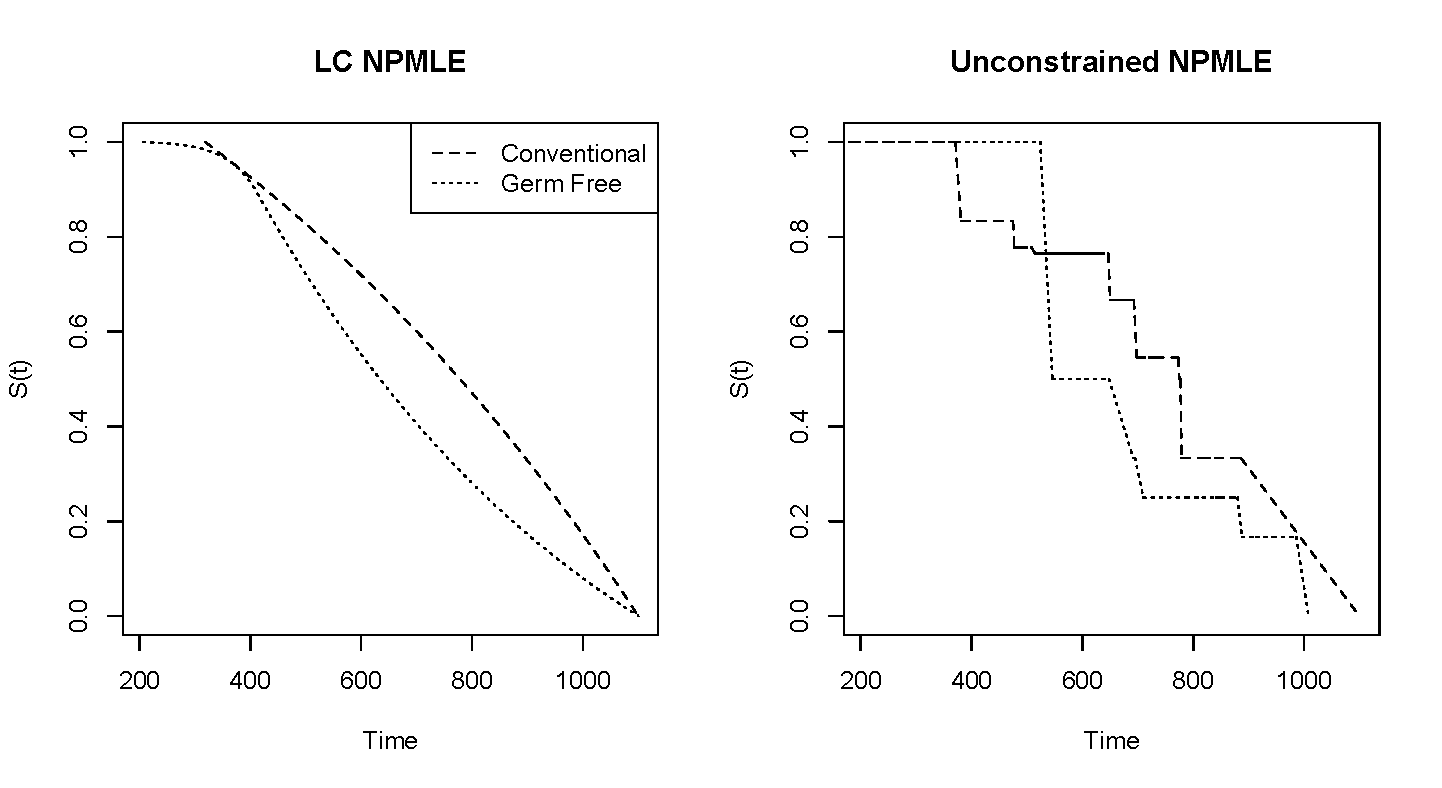
\includegraphics[width = 10cm]{TumorPlots.pdf}}
\caption{Estimated Survival Functions}
\end{figure}		

	The difference in medians as estimated by the unconstrained NPMLE was found to be 229, while the LC NPMLE estimated the difference as 144. Standard deviations for the estimated difference of medians under the null were estimated at 58.6 and 42.7 respectively, leading to z-statistics of 3.91 and 3.37. Visual examination of the sampled medians suggested the estimates were approximately normally distributed for LC NPMLE, although the unconstrained NPMLE did not appear normal. The unconstrained NPMLE is known to be not normal, but little is known about the LC NPMLE.

\begin{figure}
\centerline{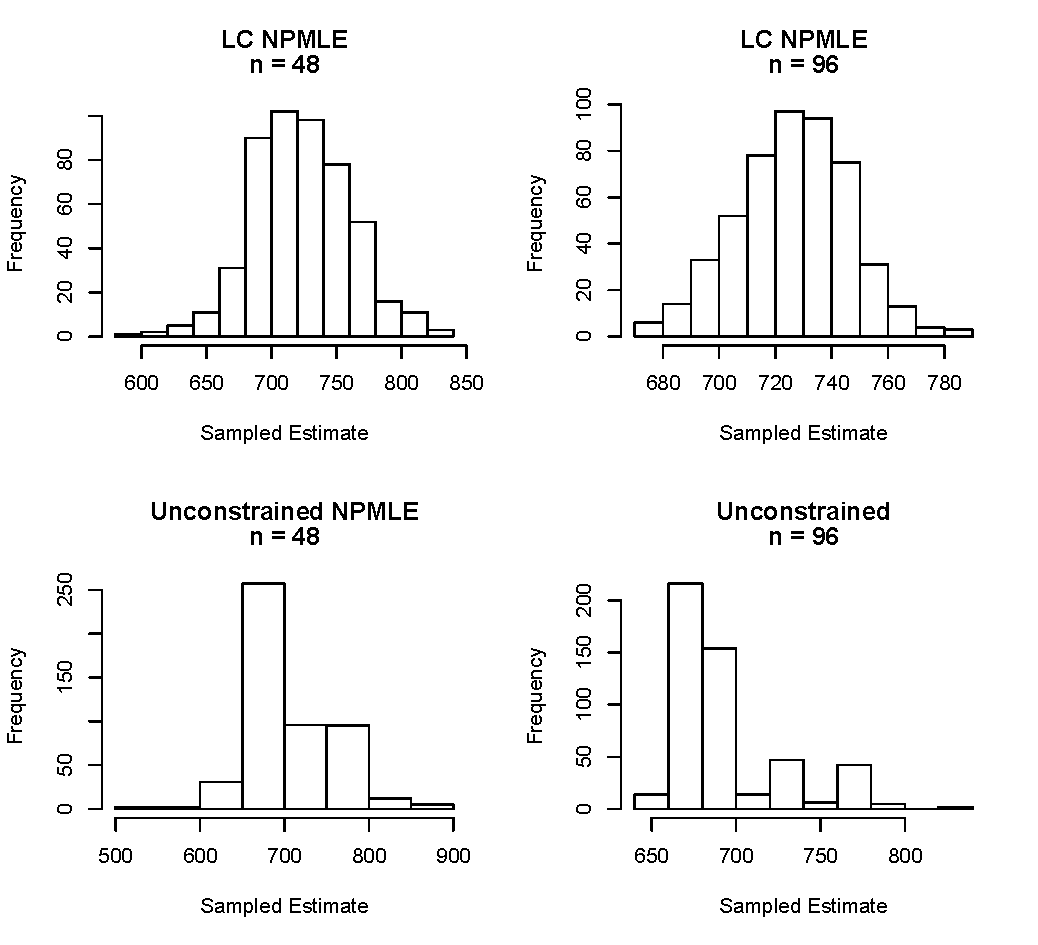
\includegraphics[width = 8cm]{MedianHist.pdf}}
\caption{Sampled Medians under the Sharp Null}
\end{figure}		

	It is worth noticing that by assuming log-concavity, our standard error was reduced approximately 27\%. If we look at the null samples of the groups individually, we see that the standard deviation of n = 48 group is estimated at 49.1 for the unconstrained estimator and 37.6 for the LC NPMLE and with the n = 96 group, we see that the estimated standard deviation 32.0 and 20.2 respectively. Thus, when the sample size increases, the gain the LC NPMLE has appears to increase to almost 37\%. This supports theory which states that the unconstrained NPMLE has a very slow rate of convergence (asymptotically $n^{-1/3}$). However, further studies should be conducted to examine the operating characteristics of both estimators in finite samples.
	
	Another interesting point that this example brings up is that of the robustness of the estimator to the assumption of log-concavity. In our case, it may be quite reasonable to believe that the true density functions are log concave for each group. However, when we take draws under the null hypothesis, we are combining our two groups. If the null hypothesis is true and the true distribution of the groups is log-concave, then the combined group will be log-concave and so we will not violate the assumption on log-concavity under the null hypothesis. An interesting note, however, is that if the alternative hypothesis is true, then we are in fact drawing from a mixture distribution which is very likely to be bimodal and thus not log-concave. While this does not affect the validity of the test, it would be of interest to know how the estimator preforms when the assumption of log-concavity is violated. Preliminary simulations appear to suggest that while some bias does occur when estimating the median for non log concave distributions, this bias appears fairly minor and the LC NPMLE substantially out preforms the unconstrained NPMLE in terms of MSE, even in moderate (n = 300) sample sizes. Further examination is required, however.



	{\subsection{Jittering the Support Points} } 
	
	As noted above, the exact location of the $m_k$ cannot be known without $\hat\phi(x)$ being known. In order to compensate for this, one can try moving the active support points between the surrounding support points in order to find the location of a knot that maximizes the log likelihood. However, because the knots will be finely partitioned for even a small data set (unless there is a very large number of ties, perhaps due to heavy rounding), the amount of movement of the knots will be very small and thus have very little effect on the log likelihood and estimated densities. Because of this, jittering should be considered to be fairly expensive in terms of computation time and done fairly infrequently, and perhaps ignored unless there is a large number of ties in the data.
